\documentclass[tikz,border=10pt]{standalone}
\usepackage{pgfplots}
\pgfplotsset{compat=1.16}

\begin{document}

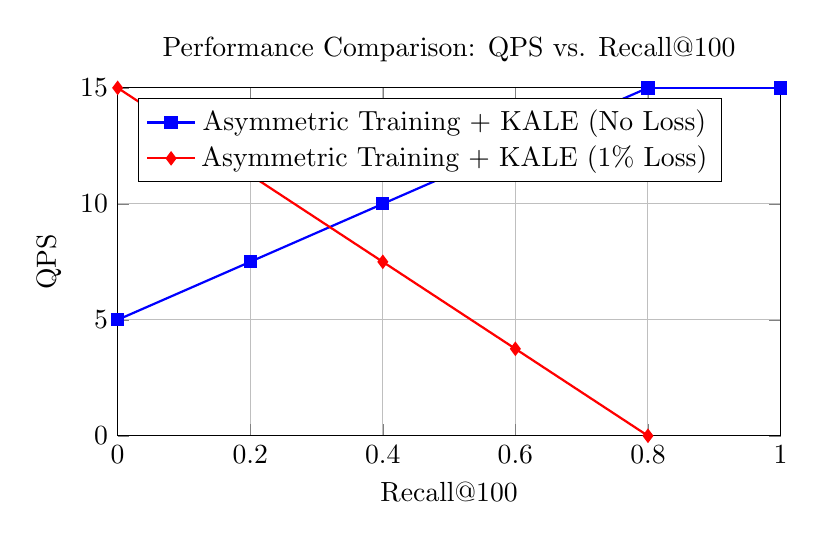
\begin{tikzpicture}
    \begin{axis}[
        title={Performance Comparison: QPS vs. Recall@100},
        xlabel={Recall@100},
        ylabel={QPS},
        ymin=0,
        ymax=15,
        xmin=0,
        xmax=1,
        xtick={0, 0.2, 0.4, 0.6, 0.8, 1},
        ytick={0, 5, 10, 15},
        grid=major,
        legend pos=north west,
        width=10cm,
        height=6cm
    ]
        \addplot[blue, mark=square*, thick] coordinates {
            (0, 5)
            (0.2, 7.5)
            (0.4, 10)
            (0.6, 12.5)
            (0.8, 15)
            (1, 15)
        };
        \addlegendentry{Asymmetric Training + KALE (No Loss)}

        \addplot[red, mark=diamond*, thick] coordinates {
            (0, 15)
            (0.2, 11.25)
            (0.4, 7.5)
            (0.6, 3.75)
            (0.8, 0)
            (1, -1.5)
        };
        \addlegendentry{Asymmetric Training + KALE (1\% Loss)}
    \end{axis}
\end{tikzpicture}

\end{document}